\documentclass[a4paper,10pt]{article}
\usepackage[utf8]{inputenc}
\usepackage[spanish]{babel}
\usepackage[affil-it]{authblk}
\usepackage{enumerate}
\usepackage{graphicx}
\usepackage{hyperref}
\usepackage{amsmath}
\usepackage{amssymb}
\usepackage{cancel}
\usepackage[usenames, dvipsnames]{color}
\usepackage{tikz}
\usepackage{multimedia}
\usepackage{subcaption} %Multiple images
\usepackage{multicol} % Multiple columns
\usepackage{float}
\usepackage{cleveref}
\usepackage[margin=1.4in]{geometry}
\usepackage[labelfont=bf]{caption}
\usepackage[titletoc,toc,title]{appendix}
\usetikzlibrary{calc}
\numberwithin{equation}{section}

%Appendices in spanish
\renewcommand{\appendixname}{Ap\'endices}
\renewcommand{\appendixtocname}{Ap\'endices}
\renewcommand{\appendixpagename}{Ap\'endices}

%Columns separation
\setlength{\columnsep}{1cm}

%Indentation
\setlength{\parindent}{0ex}

%Multiple References

\usepackage{xparse}
\ExplSyntaxOn
\NewDocumentCommand{\mref}{m}{\quinn_mref:n {#1}}
\seq_new:N \l_quinn_mref_seq
\cs_new:Npn \quinn_mref:n #1
 {
  \seq_set_split:Nnn \l_quinn_mref_seq { , } { #1 }
  \seq_pop_right:NN \l_quinn_mref_seq \l_tmpa_tl
  ( % print the left parenthesis
  \seq_map_inline:Nn \l_quinn_mref_seq
    { \ref{##1},\nobreakspace } % print the first references
  \exp_args:NV \ref \l_tmpa_tl 
  ) 
 }
\ExplSyntaxOff


%Boxes

\newcommand*{\boxcolor}{blue}
\makeatletter
\renewcommand{\boxed}[1]{\textcolor{\boxcolor}{%
\tikz[baseline={([yshift=-1ex]current bounding box.center)}] \node [rectangle, minimum width=1ex,rounded corners,draw] {\normalcolor\m@th$\displaystyle#1$};}}
 \makeatother

%Constantes
\newcommand{\euler}{\mathrm{e}}
\newcommand{\im}{i}

%Lemas, teoremas, definiciones y pruebas
\newcommand{\definicion}{\textbf{Definición: }}
\newcommand{\lema}{\textbf{Lema: }}
\newcommand{\teorema}{\textbf{Teorema: }}
\newcommand{\prueba}{\textbf{Prueba: }}


%opening
\title{Mecánica Clásica Tarea \# 6}
\author{Favio Vázquez\thanks{Correo: favio.vazquezp@gmail.com}}\affil{Instituto de Ciencias Nucleares. Universidad Nacional Autónoma de México.}
\date{}

\begin{document}

\makeatletter
\def\@maketitle{%
  \newpage
  \null
  \vskip 2em%
  \begin{center}%
  \let \footnote \thanks
    {\Large\bfseries \@title \par}%
    \vskip 1.5em%
    {\normalsize
      \lineskip .5em%
      \begin{tabular}[t]{c}%
        \@author
      \end{tabular}\par}%
    \vskip 1em%
    {\normalsize \@date}%
  \end{center}%
  \par
  \vskip 1.5em}
\makeatother

\maketitle

\section{Problema 1}

Una partícula de masa $m$ se mueve constreñida a la superficie de un paraboloide de 
revolución que tiene su abertura hacia arriba en presencia del campo de la gravedad. 
Calcule las fuerzas de constricción.

\vspace{.3cm}

\underline{Solución:} \vspace{.3cm}

Para visualizar mejor el problema al cual nos enfrentamos, se muestra en la figura 
de abajo una partícula de masa $m$ constreñida a moverse en dicho paraboloide.

\begin{figure}[H]
 \center 
 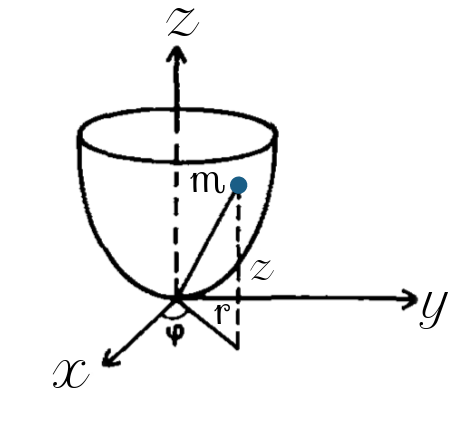
\includegraphics[scale=0.5]{problema1fig1}
 \caption{Partícula de masa $m$ se mueve constreñida a la superficie de un paraboloide de 
revolución.}
\label{fig:problema1fig1}
\end{figure}

Debido a las simetrías involucradas en este problema, utilizaremos coordenadas cilíndricas 
polares para resolverlo. Tenemos entonces las siguientes transformaciones de coordenadas,

\begin{align}
 x &= r\cos{\phi}, \\
 y &= r\sen{\phi}, \\
 z &= z.
 \label{eq:transfCoordenadasParab}
\end{align}

Por otra parte, tenemos la constricción holonómica de que la partícula debe moverse 
en la superficie del paraboloide de revolución, que podemos expresar como

\begin{equation}
 x^2 + y^2 = \alpha z.
\end{equation}

Pero en las coordenadas que estamos utilizando

\begin{equation}
 x^2 + y^2 = r^2,
\end{equation}

entonces la constricción se convierte en,

\begin{equation}
 \xi(r,\phi,z) \equiv - r^2 + \alpha z = 0.
 \label{eq:constriccionParab}
\end{equation}

Siguiendo la receta lagrangiana calculemos ahora la energía cinética y la potencial 
en nuestras coordenadas generalizadas $(r,\phi,z)$. Recordemos que podemos escribir 
estas energías en coordenadas cartesianas como,

\begin{equation}
 T = \frac{1}{2}m(\dot{x}^2 + \dot{y}^2 +\dot{z}^2).
 \label{eq:energCinetParab1}
\end{equation}

\begin{equation}
 V = mgz.
 \label{eq:energPotenParab1}
\end{equation}

Debido a que la partícula se encuentra en un campo gravitacional uniforme. Expresemos 
ahora estas energías en términos de nuestras coordenadas generalizadas. Cabe resaltar 
que utilizaremos el método de los multiplicadores indeterminados de Lagrange para obtener 
las fuerzas generalizadas, por lo cual haremos uso de la constricción en los momentos 
indicados por esta metodología. 

\vspace{.3cm}

Comencemos por obtener las derivadas temporales de \mref{eq:transfCoordenadasParab}, 
para introducirlas en \mref{eq:energCinetParab1},

\begin{align}
 \dot{x} &= \dot{r}\cos{\phi} - r \dot{\phi}\sen{\phi}, \\
 \dot{y} &= \dot{r}\sen{\phi} + r \dot{\phi}\cos{\phi}, \\
 \dot{z} &= \dot{z}.
 \label{eq:derivTemprTransfCoordParab}
\end{align}

Introduciendo \mref{eq:derivTemprTransfCoordParab} en \mref{eq:energCinetParab1} obtenemos,

\begin{align}
 \begin{split}
  T &= \frac{1}{2}m [( \dot{r}\cos{\phi} - r \dot{\phi}\sen{\phi})^2
  + (\dot{r}\sen{\phi} + r \dot{\phi}\cos{\phi})^2 + \dot{z}^2], \\
  %  
  &= \frac{1}{2} m (\dot{r}^2\cos^2{\phi} - \cancel{2r\dot{r}\dot{\phi}\cos{\phi}\sen{\phi}} + 
  r^2\dot{\phi}^2 \sen^2{\phi} +  \dot{r}^2\sen^2{\phi} \\
  %
  &+ \cancel{2r\dot{r}\dot{\phi}\cos{\phi}\sen{\phi}}
  + r^2\dot{\phi}^2 \cos^2{\phi} + \dot{z}^2 ), \\
  %
  &= \frac{1}{2} m \left[ \dot{r}^2\cancelto{1}{(\sen^2{\phi} + \cos^2{\phi})}
  + r^2\dot{\phi}^2 \cancelto{1}{(\sen^2{\phi} + \cos^2{\phi})} + \dot{z}^2 \right],
  %%
 \end{split}
\end{align}

\begin{equation}
 \therefore T = \frac{1}{2}m(\dot{r}^2 + r^2\dot{\phi}^2 + \dot{z}^2).
 \label{eq:energCinetParab2}
\end{equation}

Entonces la lagrangiana del sistema sería

\begin{equation}
 L = \frac{1}{2} m(\dot{r}^2 + r^2\dot{\phi}^2 + \dot{z}^2) - mgz.
\end{equation}

Ahora utilizando el hecho de que las ecuaciones de Lagrange en la metodología de 
multiplicadores indeterminados, se convierten en,

\begin{equation}
  \frac{d}{dt}\frac{\partial L}{\partial \dot{q}^j} - \frac{\partial L}{\partial q^j}  
 - \sum_k \lambda_k(t) \frac{\partial \xi_k}{\partial q^j} = 0,
\end{equation}

y que las fuerzas generalizadas de constricción se encuentran con

\begin{equation}
 Q_j = \sum_k \lambda_k(t) \frac{\partial \xi_k}{\partial q^j}.
 \label{eq:fuerzasConstri1}
\end{equation}

estamos en posición para aplicar el método y obtener estas fuerzas. Tendremos entonces 
las siguientes ecuaciones para $r$, $z$ y $\phi$

\begin{equation}
 \frac{d}{dt}\frac{\partial L}{\partial \dot{r}} - \frac{\partial L}{\partial r}
 - \lambda \frac{\partial \xi}{\partial r} = 0,
\end{equation}

\begin{equation}
 \frac{d}{dt}\frac{\partial L}{\partial \dot{z}} - \frac{\partial L}{\partial z}
 - \lambda \frac{\partial \xi}{\partial z} = 0,
\end{equation}

\begin{equation}
 \frac{d}{dt}\frac{\partial L}{\partial \dot{\phi}} - \frac{\partial L}{\partial \phi}
 - \lambda \frac{\partial \xi}{\partial \phi} = 0.
\end{equation}

Entonces tenemos para $r$,

\begin{equation}
  \frac{d}{dt}(m\dot{r}) - m r\dot{\phi}^2 + 2 r = 0,
\end{equation}

\begin{equation}
 \boxed{m(\ddot{r} - r\dot{\phi}^2) + 2 \lambda r = 0}.
 \label{eq:ecuMovimientoR}
\end{equation}

Para $z$,

\begin{equation}
 \frac{d}{dt}(m\dot{z}) + mg + \lambda \alpha = 0.
\end{equation}

\begin{equation}
 \boxed{m(\ddot{z}+g) + \lambda \alpha = 0 }.
 \label{eq:ecuMovimientoZ}
\end{equation}

Y para $\phi$,

\begin{equation}
 \frac{d}{dt}(mr^2\dot{\phi}) = 0.
\end{equation}

\begin{equation}
 \boxed{mr^2\dot{\phi} = \text{constante} = l}.
 \label{eq:ecuMovimientoPhi}
\end{equation}

Donde como puede verse debido a que $\phi$ es una coordenada cíclica, encontramos 
una integral de movimiento a la cual asociamos el momentum angular, el cual se 
conserva durante el movimiento de la partícula.

\vspace{.3cm}

Para poder hallar las fuerzas de constricción debemos encontrar un valor para 
$\lambda$, lo cual podemos hacer utilizando la ecuación para la constricción 
\mref{eq:constriccionParab} y vemos que 

\begin{equation}
 \alpha z = r^2,
\end{equation}

\begin{equation}
\alpha \dot{z} = 2r \dot{r},
\end{equation}

\begin{equation}
\alpha \ddot{z} = 2(\dot{r}^2 + r\ddot{r}),
\end{equation}

\begin{equation}
 \therefore \ddot{z} = 2 \frac{(\dot{r}^2 + r\ddot{r})}{\alpha}.
 \label{eq:derivConstriccionParab}
\end{equation}

Pero por la ecuación \mref{eq:ecuMovimientoZ} y usando \mref{eq:derivConstriccionParab}
vemos que,

\begin{equation}
 \ddot{z} = 2 \frac{(\dot{r}^2 + r\ddot{r})}{\alpha} = - \frac{\lambda \alpha}{m} - g,
\end{equation}

entonces,

\begin{equation}
 \ddot{r} = - \frac{\lambda \alpha^2}{2mr} - \frac{g\alpha}{2r} - \frac{\dot{r}^2}{r}.
\label{eq:doblederivR}
\end{equation}

Ahora sustituyendo \mref{eq:doblederivR} en \mref{eq:ecuMovimientoR}, y utilizando 
el hecho que $\dot{\phi}^2 = l^2/m^2r^4$ obtenemos

\begin{equation}
 m(- \frac{\lambda \alpha^2}{2mr} - \frac{g\alpha}{2r} - \frac{\dot{r}^2}{r}.
 - \frac{l^2}{m^2r^3}) + 2\lambda r = 0.
\end{equation}

Reescribiendo y agrupando términos de $\lambda$ vemos que

\begin{equation}
 - \frac{\lambda \alpha^2}{2r} + 2 \lambda r = \frac{gm\alpha}{2r} + \frac{2m\dot{r}^2}{r}
 - \frac{l^2}{mr^3},
\end{equation}

\begin{equation}
 \lambda \left(2r - \frac{\alpha^2}{2r}\right) = \frac{gm\alpha}{2r} + \frac{2m\dot{r}^2}{r}
 - \frac{l^2}{mr^3},
\end{equation}

\begin{equation}
 \lambda \left(\frac{4r^2 - \alpha^2}{2r}\right) = \frac{gm\alpha}{2r} + \frac{2m\dot{r}^2}{r}
 - \frac{l^2}{mr^3},
\end{equation}

\begin{equation}
 \lambda(4r^2 - \alpha^2) = gm\alpha + 4 m\dot{r}^2 - \frac{2l^2}{mr^2},
\end{equation}

\begin{equation}
 \boxed{\lambda = \frac{1}{4r^2 - \alpha^2} \left[ m(g\alpha + 4 \dot{r}^2) - \frac{2l^2}{mr^2}\right]}.
\end{equation}

Ahora utilizando \mref{eq:fuerzasConstri1} podemos encontrar las fuerzas generalizadas 
que serán,

\begin{equation}
 \boxed{Q_r = \lambda \frac{\partial \xi}{\partial r} = - 2r\lambda = 
 - \frac{2r}{4r^2 - \alpha^2} \left[ m(g\alpha + 4 \dot{r}^2) - \frac{2l^2}{mr^2}\right],}
\end{equation}

\begin{equation}
 \boxed{Q_z = \lambda \frac{\partial \xi}{\partial z} = \lambda \alpha = 
 \frac{\alpha}{4r^2 - \alpha^2} \left[ m(g\alpha + 4 \dot{r}^2) - \frac{2l^2}{mr^2}\right],}
\end{equation}

y 

\begin{equation}
 \boxed{Q_{\phi} = \lambda \frac{\partial \xi}{\partial \phi} = \lambda \cdot (0) = 0.}
\end{equation}






















\section{Problema 2}

Considere la lagrangiana de una partícula de masa $m$ totalmente libre en el 
espacio tridimensional desde la perspectiva de un sistema inercial y desde la 
perspectiva de un sistema que está en rotación respecto al inercial, y en 
traslación respecto a la partícula (estos movimientos no son necesariamente uniformes). 
Establezca las ecuaciones de Lagrange en ambos sistemas y, a partir de estas ecuaciones, 
encuentre las expresiones para las fuerzas ficticias; identifique en particular 
las fuerzas: centrífuga, de Coriolis, y de Euler.

\vspace{.3cm}

\underline{Solución:} \vspace{.3cm}

Como el enunciado establece que la partícula está totalmente libre en el espacio
tridimensional, entonces esto quiere decir que no está sujeta a ningún potencial, 
por lo tanto la lagrangiana para el sistema no primado será

\begin{equation}
 L = \frac{1}{2}m (\dot{r}_{S})^2.
 \label{eq:lagrangianaEnS}
\end{equation}

Sea $S'$ un sistema de referencia en rotación y traslación con respecto a un sistema inercial 
$S'$. Consideraremos que ni la traslación o la rotación son constantes, por lo que el sistema 
$S'$ puede considerarse como rotando con una velocidad angular $\mathbf{\omega}$ con respecto a
$S$ y acelerado con respecto al mismo. Denotaremos por $\mathbf{D}(t)$ al vector 
de posición del origen $O'$ relativo a $O$.

\vspace{.3cm}

Tenemos entonces que la posición de una partícula en $S$ relativa $S'$ será,

\begin{equation}
 \mathbf{r = r' + D}.
\end{equation}

Y la velocidad será,

\begin{equation}
 \mathbf{\dot{r}}_S = \mathbf{\dot{r}}'_S + \mathbf{\dot{D}},
\end{equation}

pero como $S'$ está en rotación\footnote{Si consideramos el vector de posición expresado en términos de 
las coordenadas de $S'$, 

\begin{equation*}
 \mathbf{r} = x'\mathbf{\hat{x}'} + y'\mathbf{\hat{y}'} + z'\mathbf{\hat{z}'}.
\end{equation*}

La velocidad relativa a $S'$ será 

\begin{equation*}
 \left( \frac{d\mathbf{r}}{dt} \right)_{S'} = \frac{dx'}{dt}\mathbf{\hat{x}'} 
 + \frac{dy'}{dt}\mathbf{\hat{y}'} + \frac{dz'}{dt}\mathbf{\hat{y}'}.
\end{equation*}

Relativo a $S$ ambas componentes y los vectores unitarios en la ecuación anterior 
cambian, entonces

\begin{equation*}
 \left( \frac{d\mathbf{r}}{dt} \right)_{S} = \frac{dx'}{dt}\mathbf{\hat{x}'} 
 + \frac{dy'}{dt}\mathbf{\hat{y}'} + \frac{dz'}{dt}\mathbf{\hat{y}'} + 
 x'\frac{d\mathbf{\hat{x}}}{dt} + y'\frac{d\mathbf{\hat{y}}}{dt} + z'\frac{d\mathbf{\hat{z}}}{dt}.
\end{equation*}

Pero puede probarse que \cite{delange}

\begin{equation*}
 \frac{d\mathbf{\hat{x}}}{dt} = \mathbf{\omega} \times \mathbf{\hat{x}}', \qquad 
 \frac{d\mathbf{\hat{y}}}{dt} = \mathbf{\omega} \times \mathbf{\hat{y}}', \qquad 
 \frac{d\mathbf{\hat{z}}}{dt} = \mathbf{\omega} \times \mathbf{\hat{z}}'
\end{equation*}}

\begin{equation}
 \mathbf{\dot{r}}'_S = \mathbf{\dot{r}}{'}_{S'} - \mathbf{\omega} \times \mathbf{r}'_{S'}.
\end{equation}

Tenemos entonces la siguiente fórmula de transformación de velocidades entre 
los sistemas,

\begin{equation}
 \mathbf{\dot{r}}_S = \mathbf{\dot{r}}'_{S'} - \mathbf{\omega} \times \mathbf{r}'_{S'} + \mathbf{\dot{D}}.
\end{equation}

o en notación escalar,

\begin{equation}
 \dot{r}_S  = \dot{r}'_{S'} - \omega r'_{S'} + \dot{D}.
\end{equation}

Ahora, tomando el cuadrado de esta ecuación obtenemos,

\begin{equation}
 \dot{r}_S^2 = (\dot{r}'_{S'})^2 - 2 \dot{r}'_{S'}\omega r'_{S'} + 2 \dot{r}'_{S'}\dot{D} + 
 \omega^2 {r'_{S'}}^2 - 2 \omega r'_{S'}\dot{D} + \dot{D}^2.
\end{equation}

Ahora debido a que 

\begin{equation}
 \dot{r}'_{S'}\dot{D} = \frac{d}{dt}(r'_{S'}\dot{D}) - r'_{S'}\ddot{D},
 \label{eq:lagrangeTeoremita}
\end{equation}

y recordando que una derivada con respecto al tiempo de una función de las coordenadas 
puede ser omitida de la lagrangiana porque no afecta a las ecuaciones de Lagrange, entonces 
podemos eliminar el primer término de \mref{eq:lagrangeTeoremita}, y de forma similar 
a $\dot{D}^2$ y el término $\omega r'_{S'}\dot{D}$, quedándonos entonces la siguiente ecuación,

\begin{equation}
 \dot{r}_S^2 = \dot{r}_{S'}^2 - 2 \dot{r}'_{S'}\omega r'_{S'} - 2 r'_{S'}\ddot{D}+ 
 \omega^2 r'^2.
\end{equation}

Entonces la lagrangiana en el sistema primado será,

\begin{equation}
 L' = \frac{1}{2}m [(\dot{r}'_{S'})^2 - 2 \dot{r}'_{S'}\omega r'_{S'} - 2 r'_{S'}\ddot{D}+ 
 \omega^2 {r'_{S'}}^2].
\end{equation}

Ahora que hemos encontrado la lagrangiana para el sistema primado podemos utilizar 
las ecuaciones de Lagrange para hallar las expresiones para las fuerzas ficticias 
solicitadas. Recordando que las ecuaciones de Lagrange pueden escribirse, para el 
sistema primado, como (\textbf{donde abreviaremos solo a cantidades primadas entendiendo 
que se trata a cantidades primadas en $S'$})

\begin{equation}
 \frac{d}{dt}\frac{\partial L'}{\partial \dot{r}'} - \frac{\partial L'}{\partial r'} = 0,
\end{equation}

encontramos que 

\begin{equation}
 \frac{d}{dt}(m\dot{r}' + m\omega r') - (- m \dot{r}' \omega - m\ddot{D} + mr'\omega^2) = 0,
\end{equation}

\begin{equation}
 m\ddot{r}' + m\dot{r}'\omega + mr'\dot{\omega} + m \dot{r}' \omega  + m\ddot{D} 
 -  mr'\omega^2 = 0.
\end{equation}

\begin{equation}
 \boxed{m\ddot{r}' = - m r'\dot{\omega} - 2m \dot{r}' \omega + m\ddot{D} +  mr'\omega^2.}
\label{eq:finalRotacionTraslacion}
 \end{equation}

De la ecuación \mref{eq:finalRotacionTraslacion} podemos ver claramente los términos 
de las fuerzas pedidas, el término $ 2m \dot{r}' \omega$ es el de la fuerza de Coriolis, 
el término $mr'\omega^2$ es el de la fuerza centrífuga, y el término $mr'\dot{\omega}$ 
es el de la fuerza de Euler; el término $m\ddot{D}$ se conoce como la fuerza traslacional 
y surge por el hecho que hemos considerado que el sistema primado puede moverse de 
manera no uniforme, lo mismo ocurre con la fuerza de Euler (o fuerza Azimutal) que surge 
por el hecho de que hemos considerado que la rotación puede ser no uniforme.

\vspace{.3cm}

Para completar el entendimiento de este ejercicio, quisimos hacer un ejemplo concreto, no 
tan general como el resultado que hemos obtenido anteriormente, para ver de que forma 
surgen estas fuerzas en un problema más específico. Consideraremos el caso particular 
de un sistema en rotación, y no en traslación con respecto al sistema inercial. La imagen de abajo representa a los dos sistemas con los que trataremos, el primero que 
es no primado será un sistema de coordenadas cartesianas inercial y el segundo que 
está primado será el sistema en rotación. En este caso consideremos un sistema 
no inercial que está en rotación en sentido de las agujas del reloj sobre el eje $z$, y para  ser completos
en la demostración y  acatar lo establecido en el enunciado,  asumiremos que el
ángulo de rotación $\theta$ es una función dada del tiempo $\theta = \theta(t)$.

\begin{figure}[H]
 \center 
 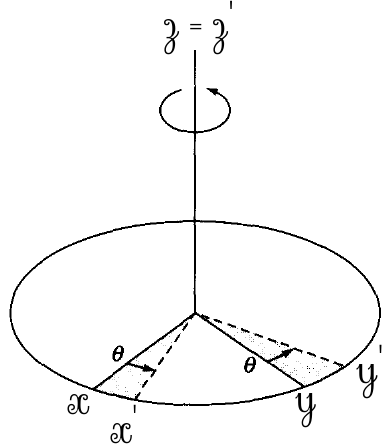
\includegraphics[scale=0.44]{problema2fig1}
 \caption{Rotación del sistema de coordenadas $(x,y,z)$ en dirección de las agujas 
 del reloj sobre el eje $z$ con un ángulo $\theta(t)$.}
 \label{fig:problema2fig1}
\end{figure}

De nuevo, como el enunciado establece que la partícula está totalmente libre en el espacio
tridimensional, entonces esto quiere decir que no está sujeta a ningún potencial, 
por lo tanto la lagrangiana para el sistema no primado será

\begin{equation}
 L = \frac{1}{2}m (\dot{x}^2 + \dot{y}^2 + \dot{z}^2).
\end{equation}

Por otra parte, la matriz de rotación será 

\begin{equation}
 \lambda = \begin{pmatrix}
          \cos{\theta} & \sen{\theta} & 0 \\
          -\sen{\theta} & \cos{\theta} & 0 \\
          0 & 0 & 1
          \end{pmatrix}.
\end{equation}

Por lo tanto tendremos las siguientes transformaciones entre los sistemas, una 
para ir de los primados a los no primados

\begin{align}
 x' &= x\cos{\theta} + y \sen{\theta}, \\
 y' &= -x\sen{\theta} + y\cos{\theta}, \\
 z' &= z,
\end{align}

y una para ir de los no primados a los primados

\begin{align}
 x &= x'\cos{\theta} - y' \sen{\theta}, \\
 y &= x'\sen{\theta} + y'\cos{\theta}, \\
 z &= z',
 \label{eq:transfCoordNonInertial}
\end{align}

Debido a que las necesitaremos en la lagrangiana para el sistema primado, obtengamos 
las primeras derivadas temporales de las ecuaciones \mref{eq:transfCoordNonInertial}

\begin{align}
 \dot{x} &= \dot{x}'\cos{\theta} - x'\dot{\theta}\sen{\theta} - \dot{y}'\sen{\theta} - y'\dot{\theta}\cos{\theta}, \\
 \dot{y} &= \dot{x}'\sen{\theta} + x'\dot{\theta}\cos{\theta} + \dot{y}'\cos{\theta} - y'\dot{\theta}\sen{\theta}, \\
 \dot{z} &= \dot{z}'.
 \label{eq:derivTransfNonInertial1}
\end{align}

Si llamamos a $\dot{\theta} = \omega$, a la cual asociamos la velocidad angular de 
la rotación, entonces las ecuaciones \mref{eq:derivTransfNonInertial1} se convierten en

\begin{align}
  \dot{x} &= \dot{x}'\cos{\theta} - \omega x'\sen{\theta} - \dot{y}'\sen{\theta} - \omega y'\cos{\theta}, \\
 \dot{y} &= \dot{x}'\sen{\theta} + \omega x'\cos{\theta} + \dot{y}'\cos{\theta} - \omega y'\sen{\theta}, \\
 \dot{z} &= \dot{z}'.
 \label{eq:derivTransfNonInertial2}
\end{align}

Podemos escribir \mref{eq:derivTransfNonInertial2} de una forma más compacta,

\begin{align}
 \dot{x} &= (\dot{x}' - \omega y')\cos{\theta} - (\dot{y}' + \omega x')\sen{\theta}, \\
 \dot{y} &= (\dot{y}' + \omega x')\cos{\theta} + (\dot{x}' - \omega y')\sen{\theta}, \\
 \dot{z} &= \dot{z}'.
\end{align}

Entonces la lagrangiana en el sistema primado será

\begin{align}
\begin{split}
 L' & = \frac{1}{2}m\{[(\dot{x}' - \omega y')\cos{\theta} - (\dot{y}' + \omega x')\sen{\theta}]^2 \\ 
 &+ [(\dot{y}' + \omega x')\cos{\theta} + (\dot{x}' - \omega y')\sen{\theta}]^2 + (\dot{z}')^2\}.
 \end{split}
\end{align}

Trabajando el álgebra para estos términos tendremos,

\begin{align*}
 L' &= \frac{1}{2}m [(\dot{x}' - \omega y')^2\cos^2{\theta} - \cancel{2(\dot{x}' - \omega y')(\dot{y}' + \omega x')\cos{\theta}\sen{\theta}} \\
    &+ (\dot{y}' + \omega x')^2\sen^2{\theta} + (\dot{y}' + \omega x')^2\cos^2{\theta} \\
    &+ \cancel{2(\dot{x}' - \omega y')(\dot{y}' + \omega x')\cos{\theta}\sen{\theta}} + (\dot{x}' - \omega y')^2\sen^2{\theta} \\
    &+ (\dot{z}')^2].
\end{align*}

\begin{align*}
 L' &= \frac{1}{2}m [(\dot{x}' - \omega y')^2\cos^2{\theta} + (\dot{y}' + \omega x')^2\sen^2{\theta} + (\dot{y}' + \omega x')^2\cos^2{\theta} \\ 
    &+ (\dot{x}' - \omega y')^2\sen^2{\theta} + (\dot{z}')^2 ].
\end{align*}

\begin{equation*}
 L' = \frac{1}{2}m \left[(\dot{x}' - \omega y')^2\cancelto{1}{(\sen^2{\theta} + \cos^2{\theta})} + 
 (\dot{y}' + \omega x')^2\cancelto{1}{(\sen^2{\theta} + \cos^2{\theta})} + (\dot{z}')^2 \right].
\end{equation*}

\begin{equation*}
 L' = \frac{1}{2}m \left[(\dot{x}' - \omega y')^2 + (\dot{y}' + \omega x')^2  + (\dot{z}')^2\right].
\end{equation*}

\begin{equation*}
 L' = \frac{1}{2}m \left[ (\dot{x}')^2 - 2\omega \dot{x}'y' + \omega^2(\dot{y}')^2 + 
 (\dot{y}')^2 + 2\omega\dot{y}'x' + \omega^2(\dot{x}')^2 + (\dot{z}')^2 \right].
\end{equation*}

\begin{equation}
 \boxed{L' = \frac{1}{2}m \left[ (\dot{x}')^2 + (\dot{y}')^2 + (\dot{z}')^2 + 2\omega(\dot{y}'x' - \dot{x}'y')
 + \omega^2((\dot{y}')^2 + (\dot{x}')^2)\right]. }
\end{equation}

Ahora que hemos encontrado la lagrangiana para el sistema primado podemos utilizar 
las ecuaciones de Lagrange para hallar las expresiones para las fuerzas ficticias 
solicitadas. Recordando que las ecuaciones de Lagrange pueden escribirse, para el 
sistema primado, como

\begin{equation}
 \frac{d}{dt}\frac{\partial L'}{\partial \dot{q}^{i}{'}} - \frac{\partial L'}{\partial q^{i}{'}} = 0.
\end{equation}

Tendremos entonces las siguientes ecuaciones de movimiento:

\vspace{.3cm}

Para $x'$,

\begin{align*}
 \frac{d}{dt}(m\dot{x}' - m\omega y') - m\omega\dot{y}' - m\omega^2x' = 0, \\
 %
 m\ddot{x}' - m\omega\dot{y}' - m\dot{\omega}y' - m\omega\dot{y}' - m\omega^2x' = 0,
\end{align*}

\begin{equation}
 \boxed{m\ddot{x}' = 2m\omega\dot{y}' + m\omega^2 x'+ m\dot{\omega}y'}.
 \label{eq:ecuMoviXNonInertial}
\end{equation}

Para $y'$,

\begin{align*}
 \frac{d}{dt}(m\dot{y}' + m\omega x') + m\omega \dot{x}' - m\omega^2y' = 0, \\
 m\ddot{y}' + m\omega\dot{x}' + m\dot{\omega}x' + m\omega \dot{x}' - m\omega^2y' = 0.
\end{align*}

\begin{equation}
 \boxed{m\ddot{y}' = -2m\omega\dot{x}' + m\omega^2 y' - m\dot{\omega}x'.}
  \label{eq:ecuMoviYNonInertial}
\end{equation}

Y para $z'$

\begin{equation}
 \boxed{\frac{d}{dt}(m\dot{z}') = 0 \Rightarrow m\dot{z}' = \text{constante}.}
  \label{eq:ecuMoviZNonInertial}
\end{equation}

Podemos ahora fácilmente reconocer las fuerzas ficticias que también se encuentran en 
el tratamiento de sistemas no inerciales con la mecánica vectorial. Los términos 
proporcionales a $\omega$ son las "fuerzas de Coriolis``

\begin{equation}
\boxed{ \vec{F}' \text{(Coriolis)} = (2m\omega\dot{y}', -2m\omega\dot{x}', 0) = -2m\vec{\omega} \times \dot{\vec{r}'}.}
\end{equation}

Los términos proporcionales a $\omega^2$ son las ''fuerzas centrífugas`` 

\begin{equation}
 \boxed{\vec{F}' \text{(Centrífuga)} = ( m \omega^2 x', m\omega^2 y', 0) = - m \vec{\omega} \times (\vec{\omega} \times \vec{r}').}
\end{equation}

Y los términos proporcionales a $\dot{\omega}$ son las ''fuerzas de Euler``

\begin{equation}
 \boxed{\vec{F}' \text{(Euler)} = (m\dot{\omega}y', -m\dot{\omega}x', 0 ) = - m \dot{\vec{\omega}} \times \vec{r}'.}
\end{equation}

Con lo cual hemos comprobado que podemos llegar a las mismas expresiones para las fuerzas 
ficticias desde un marco lagrangiano a las que se encuentran con la mecánica vectorial, pero 
con mucho menos trabajo. Cabe destacar que las fuerzas de Euler surgen debido a que 
hemos considerado que la velocidad angular de rotación puede cambiar en el tiempo. Claramente 
como en este ejemplo práctico que hemos hecho no consideramos traslación, no surge 
el término de fuerza traslacional que vimos anteriormente.


\section{Problema 3}

Un girocompás es un instrumento que consisten de un cuerpo rígido simétrico, 
$(I_1 = I_2 \ne I_3)$ cuyo eje de simetría está constreñido a permanecer sobre 
un plano horizontal en la superficie de la Tierra, la que, naturalmente está en 
rotación en torno a su eje con un período de 24 horas. Suponga que un girocompás 
se encuentra en un punto de la Tierra de latitud $\phi$ y se pone, inicialmente, 
en rotación en torno a su eje de simetría con una velocidad angular $\omega_3$ cuando 
dicho eje apunta en una dirección arbitraria. Calcule una lagrangiana para este 
sistema. Demuestre que la velocidad de rotación en torno al eje de simetría, $\omega_3$,
permanece constante. Demuestre que si $\omega_3 > (I_1/I_3)\omega_0\cos{\phi}$ entonces 
el eje de simetría oscilará, de manera estable, en torno a la dirección norte-sur 
($\omega_0$ es la velocidad angular de la Tierra).

\vspace{.3cm}

\underline{Solución:} \vspace{.3cm}

\textbf{Nota}: \textbf{Debido a problemas de notación, ya que utilizaremos los 
ángulos de Euler en su forma estándar, el punto de la Tierra donde
se encuentra el girocompás tendrá una latitud $\lambda$, y no $\phi$. Además
debido a la complejidad de este problema, algunas demostraciones y resultados relevantes 
se han dejado para los apéndices. Para solucionar este problema se utilizarán análisis 
de varios libros de mecánica analítica, y se recomienda al lector interesado que se dirija 
a la bibliografía para un estudio más completo de este interesante artefacto.}

\noindent\rule[0.5ex]{\linewidth}{1pt}

\vspace{.3cm}

El girocompás es un dispositivo diseñado para determinar la rotación del norte verdadero 
(o sur verdadero). Está hecho para siempre apuntar al norte celeste de la Tierra (no como 
las brújulas magnéticas que apuntan al norte magnético de la Tierra). Esto se logra 
añadiendo un contra peso del cardán\footnote{Componente mecánico, descrito por primera vez por Girolamo
Cardano, que permite unir dos ejes no colineales. Su objetivo es transmitir el movimiento de rotación de un
eje al otro a pesar de la no colinealidad.} interno de un giroscopio, que resulta en un 
movimiento de precesión que puede ser ajustado para coincidir con la precesión de 
la Tierra. La figura de abajo, sacada de \cite{baruh} muestra una representación 
esquemática del girocompás; como establece \cite{saletan}, los girocompases reales 
usados en los barcos o algunas aeronaves, son mucho más complicados de lo que trataremos 
acá, nos limitaremos a trabajar con un sistema idealizado (algunas de las suposiciones 
que utilizamos en esta derivación están detalladas al final del apéndice \mref{app:apendice1}).

\begin{figure}[H]
 \center 
 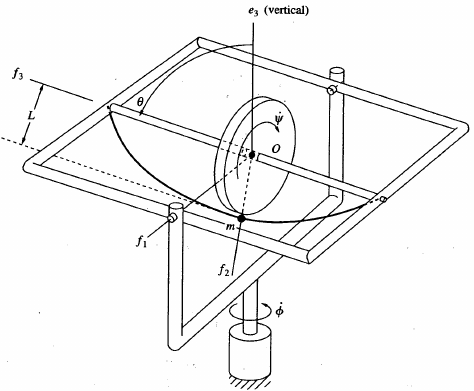
\includegraphics[scale=0.5]{problema3fig1}
 \caption{Representación esquemática de un girocompás}
 \label{fig:problema3fig1}
\end{figure}

El rotor está colocado en el medio del cardán interno y una masa oscilante $m$ está 
fijada al fondo del cardán interno. Usaremos un sistema de coordenadas $e_1e_2e_3$
fijado a la Tierra, donde $\hat{e}_1$ apunta al norte, $\hat{e}_2$ al oeste, y $\hat{e}_3$
es la vertical local (esto está explicado con detalle en el apéndice \mref{app:apendice1}). 
La velocidad angular de este sistema de coordenadas es (ver ecuación \mref{eq:velAngTierra1}) 

\begin{equation}
 \vec{\omega}_{AT} = \omega_0(\cos{\lambda}\hat{e}_1 + \sen{\lambda}\hat{e}_3),
\end{equation}

donde $\lambda$ es la latitud del punto de la Tierra donde se encuentra el girocompás, y 
$\omega_0$es la velocidad angular de la Tierra, $\omega_0 = 7.292\times 10^-5$ rad/s. 
El tratamiento del cardán interior - que llamaremos marco\footnote{Ver apéndice 
\mref{app:apendice3}.} $F$ - se obtiene de una transformación\footnote{Ver apéndice 
\mref{app:apendice2}.} $3-1$, de manera que la velocidad angular del rotor con respecto 
a la Tierra es\footnote{ver figura \mref{fig:problema3fig1} y la ecuación \mref{eq:velAngFframe3}.}

\begin{equation}
 \vec{\omega}_{TB} = \dot{\theta}\hat{f}_1 + \dot{\phi}\sen{\theta}\hat{f}_2 + 
 (\dot{\phi}\cos{\theta} + \dot{\psi})\hat{f}_3.
\end{equation}

Los vectores unitarios en el marco $T$ de la Tierra, y el marco $F$ están relacionados 
por\footnote{Ver figura \mref{fig:apendice4fig1}}

\begin{equation}
 \hat{e}_1 = \cos{\phi}\hat{f}_1 - \sen{\phi}\cos{\theta}\hat{f}_2 + \sen{\phi}\sen{\theta}\hat{f}_3 
 \qquad \hat{e}_3 = \sen{\theta}\hat{f}_2 + \cos{\theta}\hat{f}_3,
\end{equation}

por lo que podemos escribir la velocidad del rotor como\footnote{Ver ecuación 
\mref{eq:velAngFframe3}.}

\begin{equation}
 \vec{\omega}_{AB} = \vec{\omega}_{AT} + \vec{\omega}_{TB} = \omega_1\hat{f}_1 
 + \omega_2\hat{f}_2 + \omega_3\hat{f}_3,
\end{equation}

donde 

\begin{align}
 \omega_1 &= \omega_0\cos{\lambda}\cos{\phi} + \dot{\theta}, \\
 \omega_2 &= - \omega_0\cos{\lambda}\sen{\phi}\cos{\theta} + \omega_0\sen{\lambda}\sen{\theta} + 
 \dot{\phi}\sen{\theta}, \\
 \omega_3 &= \omega_0\cos{\lambda}\sen{\phi}\sen{\theta} + \omega_0\sen{\lambda}\cos{\theta} 
 + \dot{\phi}\cos{\theta} + \dot{\psi}.
\end{align}

Debido a que las tasas precesión y nutación son bajas, ignoraremos la energía 
cinética de la masa oscilante, así que la energía cinética del sistema será solo 
la debida rotor. Además, ignoraremos términos cuadráticos en $\omega_0$, debido a que 
la velocidad angular de la Tierra es muy pequeña. Como queremos ver si hay unos 
ángulos de precesión y nutación para los cuales el eje del rotor y tasa de espín 
son constantes, consideraremos la precesión y nutación como cero. Ignorando además 
la inercia de los cardanes, y recordando que para el girocompás $I_1=I_2$ tenemos 
que la energía cinética será (el álgebra no es complicada pero extensa, así que 
se omitirá de esta tarea)

\begin{equation}
 T = \frac{1}{2}I_1 (\omega_1^2 + \omega_2^2) + \frac{1}{2}\omega_3^2. \approx 
 \frac{1}{2}I_3[\dot{\psi}^2 + 2\dot{\psi}\omega_0(\cos{\lambda}\sen{\phi}\sen{\theta} + 
 \sen{\lambda}\cos{\theta})].
\end{equation}

Mientras que la energía potencial es debida solamente a la masa oscilante,

\begin{equation}
 V = - mgL\sen{\theta}.
\end{equation}

Podemos construir entonces la lagrangiana $L = T - V$ del sistema,

\begin{equation}
 \boxed{L = \frac{1}{2}I_3[\dot{\psi}^2 + 2\dot{\psi}\omega_0(\cos{\lambda}\sen{\phi}\sen{\theta} + 
 \sen{\lambda}\cos{\theta})] + mgL\sen{\theta}.}
 \label{eq:lagrangianaGirocompas}
\end{equation}

Tenemos entonces las siguientes ecuaciones de movimiento:

\vspace{.3cm}

Para $\theta$, 

\begin{equation}
 \frac{d}{dt}\frac{\partial L}{\partial \dot{\theta}} - \frac{\partial L}{\partial \theta} = 0.
\end{equation}

Pero como \mref{eq:lagrangianaGirocompas} no depende de $\dot{\theta}$, entonces 

\begin{equation}
 \frac{\partial L}{\partial \theta} = 0,
\end{equation}

entonces,

\begin{equation}
 \boxed{I_3\dot{\psi}\omega_0(\cos{\lambda}\sen{\phi}\cos{\theta} - \sen{\lambda}\sen{\theta}) 
 + mgL\cos{\theta} = 0}.
 \label{eq:movimientoTheta}
\end{equation}

Para $\phi$, 

\begin{equation}
 \frac{d}{dt}\frac{\partial L}{\partial \dot{\phi}} - \frac{\partial L}{\partial \phi} = 0.
\end{equation}

De nuevo, \mref{eq:lagrangianaGirocompas} no depende de $\dot{\phi}$, entonces 

\begin{equation}
 \frac{\partial L}{\partial \phi} = 0,
\end{equation}

entonces,

\begin{equation}
 \boxed{\dot{\phi}\omega_0\cos{\lambda}\cos{\phi}\sen{\theta} = 0.}
 \label{eq:movimientoPhi}
\end{equation}

Por último para, $\psi$, debido a que \mref{eq:lagrangianaGirocompas} no depende 
de $\psi$ tenemos que,

\begin{equation}
 \frac{d}{dt}[I_3\dot{\psi} + I_3\omega_0(\cos{\lambda}\sen{\phi}\sen{\theta} + 
 \sen{\lambda}\cos{\theta})] = 0,
\end{equation}

entonces hemos encontrado una integral de movimiento que la asociamos con el momentum 
de espín $p_{\psi}$,

\begin{equation}
 \boxed{\dot{\psi} + \omega_0(\cos{\lambda}\sen{\phi}\sen{\theta}+ 
 \sen{\lambda}\cos{\theta}) = p_{\psi}.}
 \label{eq:movimientoPsi}
\end{equation}

Ahora, estamos interesados en los valores de $\phi$ y $\theta$ que hacen a las ecuaciones
\mref{eq:movimientoTheta} y \mref{eq:movimientoPhi} válidas. Para que la segunda ecuación sea 
válida, debido a que ni $\dot{\phi}$, ni $\omega_0$, ni $\cos{\lambda}$ son iguales a
cero, entonces o $\cos{\phi} = 0$ o $\sen{\theta} = 0$. El caso en que $\sen{\theta} = 0$ 
no tiene mucho sentido estudiarlo, porque corresponde al caso en el que el cardán interno no se 
ha movido. Entonces consideramos que $\cos{\phi}= 0$. Esto es posible para $\phi= \pm \pi/2$. Por 
simplicidad nos quedaremos con el caso en que $\phi = \pi/2$ para que $\sen{\phi} = 1$. Ahora 
tomando este resultado vemos que la expresión para $\omega_3$ se transforma en,

\begin{equation}
 \omega_3 = \omega_0\cos{\lambda}\cancelto{1}{\sen{\phi}}\sen{\theta} + \omega_0\sen{\lambda}\cos{\theta} + 
 \cancelto{0}{\dot{\phi}\cos{\theta}} + \dot{\psi},
\end{equation}

\begin{equation}
 \boxed{\omega_3 = \omega_0(\cos{\lambda}\sen{\theta} + \sen{\lambda}\cos{\theta}) + \dot{\psi}.}
\end{equation}

Y haciendo lo mismo para $p_\psi$ vemos que,

\begin{equation}
 p_\psi = \omega_0(\cos{\lambda}\cancelto{1}{\sen{\phi}}\sen{\theta}+ 
 \sen{\lambda}\cos{\theta} + \dot{\psi},
\end{equation}

\begin{equation}
 \boxed{p_\psi = \omega_0(\cos{\lambda}\sen{\theta} + \sen{\lambda}\cos{\theta}) + \dot{\psi}.}
\end{equation}

\textbf{Entonces debido a que $p_\psi = \omega_3$ hemos demostrado que la velocidad de rotación 
en torno al eje de simetría permanece constante}.

\vspace{.3cm}

Para probar la última parte del problema, no o haremos directamente con lo que nos dice 
el enunciado debido a que el tratamiento que hemos hecho lleva al mismo resultado 
pero llegar a él es un poco distinto. Podemos ver esto, si introducimos estas consideraciones a la ecuación 
\mref{eq:movimientoTheta} y resolvemos para $\theta$, tenemos que 

\begin{equation}
 \cot{\theta} = \frac{I_3\dot{\psi}\omega_o\sen{\lambda}}{I_3\dot{\psi}\omega_0\cos{\lambda} + mgL}.
\label{eq:cotangenteTheta}
\end{equation}

Pero debido a que $mgL$ es mucho más grande que $I_3\dot{\psi}\omega_0$, entonces el término 
$mgL$ domina la ecuación de arriba. Además $\cot{\theta}$ es muy pequeño y $\theta$ es 
muy cercano a $\pi/2$. Introduciendo la expresión

\begin{equation}
 \theta = \frac{\pi}{2} - \Delta\theta,
\end{equation}

donde $\Delta\theta$ es pequeña, podemos simplificar la ecuación \mref{eq:cotangenteTheta}
a 

\begin{equation}
 \boxed{\Delta\theta = \frac{I_3\dot{\psi}\omega_0\sen{\lambda}}{mgl}.}
\end{equation}

Con lo cual podemos establecer que si el rotor se suelta con su eje de rotación inclinado 
a un ángulo $\Delta\theta$ sobre la horizontal norte-sur, la precesión del giroscopio 
coincidirá con la componente de la velocidad angular de la Tierra en la dirección del 
vertical local, o lo que es lo mismo, el girocompás oscilará en torno a la dirección 
norte-sur buscando el norte verdadero, en un plano horizontal.

\vspace{.3cm}

Para complementar esta discusión, puede probarse además \cite{delange}, que si llamamos $\xi$ el ángulo entre el norte 
verdadero y el eje de rotación del girocompás, tendremos la siguiente ecuación diferencial 
para $\xi$,

\begin{equation}
 \ddot{\xi} + [(I_1/I_3)\omega_3\omega_0\cos{\lambda}]\sen{\xi} = 0, 
\end{equation}

con lo que vemos que el rotor oscilará en un plano horizontal sobre el norte verdadero 
($\xi=0$), lo cual concuerda con lo que habíamos probado anteriormente. Más aún, para 
pequeñas oscilaciones $|\xi| \ll 1$ la ecuación no lineal anterior se puede 
aproximar a 

\begin{equation}
 \ddot{\xi} + [(I_1/I_3)\omega_3\omega_0\cos{\lambda}]\xi = 0, 
\end{equation}

la cual es muy similar a la de un oscilador armónico con período 

\begin{equation}
 P = 2\pi[(I_1/I_3)\omega_3\omega_0\cos{\lambda}]^{-1/2},
\end{equation}

y la oscilación será estable \cite{spivak} si $\omega_3 >(I_1/I_3)\omega_0\cos{\lambda}$, 
con lo cual hemos terminado todas las demostraciones.

\vspace{.3cm}

Al lector interesado se le recomienda dirigirse a la bibliografía donde se encontrará 
con mucha más información detallada sobre el girocompás. 

\vspace{.3cm}

Específicamente para una discusión física y teórica los libros de 
Baruh, \cite{baruh}, José y Saletan \cite{saletan}, Spivak \cite{spivak},
Chaichian et. al \cite{chaichian}, Fowles y Cassiday \cite{fowles}, Synge y Griffith \cite{synge} y Meirovitch \cite{meirovitch}. 
Para una discusión física y computacional (Mathematica) el libro de Romano \cite{romano}. Y para una discusión ingenieril y práctica los 
libros de Ginsberg \cite{ginsberg1} y \cite{ginsberg2}.

\newpage

\appendix
\appendixpage

\section{Movimiento con respecto a la Tierra} \label{app:apendice1}

\textbf{Nota}: Este apéndice es una reconstrucción de una parte de la sección 2.8 
de \cite{baruh}. 

\vspace{.3cm}

Consideremos una partícula cerca de la superficie de la Tierra, y adjuntemos un marco 
de referencia en movimiento $B$ a la superficie de la Tierra usando un sistema 
$xyz$. La dirección $z$ es la vertical, la dirección $x$ es hacia el norte y la 
dirección $y$ es hacia el oste. En las figuras de bajo se muestra un poco mejor 
la situación

\begin{figure}[H]
 \center
 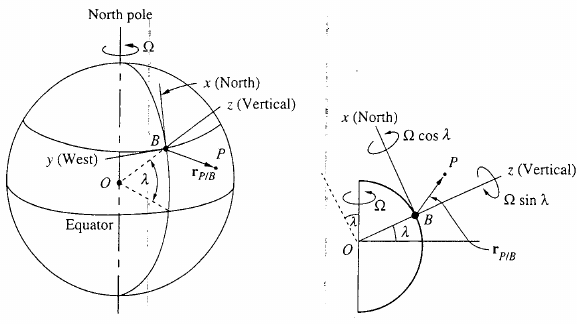
\includegraphics[scale=0.7]{apendice1fig1}
 \caption{Movimiento con respecto a la Tierra.}
  \label{fig:apendice1fig1}
\end{figure}

Asumiremos que la Tierra está rotando sobre su propio eje con una velocidad angular 
constante $\Omega$. La parte de la derecha de la figura \mref{fig:apendice1fig1} 
muestra el sistema de coordenadas visto de lado. Considerando esta figura, podemos 
describir la velocidad angular de la Tierra en forma vectorial como

\begin{equation}
 \vec{\Omega} = \Omega(\sen{\lambda}\hat{k}+\cos{\lambda}\hat{i}),
 \label{eq:velAngTierra1}
\end{equation}

donde $\lambda$ es la latitud. Hemos ignorado la velocidad angular de la Tierra. Esta 
suposición y la de que la rotación de la Tierra son constantes no son exactamente 
ciertas. La rotación de la Tierra sobre si misma no es sobre un eje fijo. El eje 
sobre el cual la Tierra rota exhibe un pequeño movimiento de bamboleo con un 
período de 433 días, principalmente porque la Tierra no es totalmente rígida, ni 
totalmente esférica. La tasa de rotación de la Tierra no es constante; se esta 
reduciendo a una tasa extremadamente pequeña. Además, ignoramos la inclinación 
entre el plano ecuatorial (el plano generado por el ecuador) y el plano eclíptico 
(el plano generado por la órbita de la Tierra alrededor del Sol). También hemos 
ignorado el movimiento relativo de Tierra con respecto al Sol.

\newpage

\section{Secuencias de Ángulos de Euler} \label{app:apendice2}

\textbf{Nota}: Este apéndice es una reconstrucción de una parte de la sección 7.5.1 
de \cite{baruh}.

\vspace{.3cm}

En este apéndice, usaremos rotaciones fijas a un cuerpo, y seleccionamos 
los ejes no-paralelos sobre los cuales se ejecutan las rotaciones como los ejes 
del marco rotado. Los tres ángulos usados para transformar un conjunto de coordenadas 
en otro, en este ámbito, se llaman los ángulos de Euler.

\vspace{.3cm}

En la generación de tres conjuntos de rotaciones para transformar un conjunto de 
coordenadas en otro, i.e., $a_1a_2a_3$ a $b_1b_2b_3$, hay doce opciones en las cuales 
no son iguales dos índices de rotación. Comenzamos con el marco $a_1a_2a_3$ y lo 
rotamos sobre uno de los ejes para obtener el marco $a'_1a'_2a'_3$. Acá tenemos 
tres opciones. La siguiente rotación es sobre uno de los ejes $a'_1$, $a'_2$ o $a'_3$, 
excluyendo el eje que coincide con con la pasada rotación. Es decir, si la primera 
rotación es sobre el eje $a_2$, la segunda rotación no debe ser sobre el eje $a'_2$. 
Entonces, tenemos dos posibles rotaciones por cada rotación previa. Seguimos el mismo 
procedimiento para la tercera transformación, resultado en dos posibles transformaciones 
para cada rotación previa. Como resultado tenemos $3 \times 2 \times 2 = 12$ posibles 
combinaciones 

\begin{align*}
 1-2-1,\quad 1-2-3,\quad 1-3-1,\quad 1-3-2,\quad 2-1-2,\quad 2-1-3, \\
 2-3-1,\quad 2-3-2,\quad 3-1-2,\quad 3-1-3,\quad 3-2-1,\quad 3-2-3.
\end{align*}

Estos doce conjuntos son llamados las \emph{secuencias de ángulos de Euler}. Pueden 
clasificarse en dos categorías principales, cada una con características similares. 
La primera categoría es cuando el primer y el tercer índice son iguales (e.g., $3-2-3$) 
y la segunda categoría consiste en rotaciones donde el primer y el tercer índice 
son diferentes (e.g., $1-2-3$). Se escoge la secuencia dependiendo de la aplicación, 
de manera tal que la secuencia escogida de una mejor visualización y conlleve a 
menos singularidades.
 
\vspace{.3cm}

Uno de las secuencias de Euler más utilizadas es la $3-1-3$, ver figura \mref{fig:apendice2fig1}, muy usada para describir 
cuerpos rígidos en rotación (es la que utilizamos para el problema del girocompás). En 
una transformación $3-1-3$, primero, los ejes $a_1a_2a_3$ se rotan sobre $a_3$ 
con un ángulo $\phi$, resultando en los ejes $a'_1a'_2a'_3$. Luego, se hace una rotación 
sobre el eje $a'_1$ con un ángulo $\theta$, produciendo los ejes $a''_1a''_2a''_3$. 
El eje $a'_1$ también es conocido como la línea de nodos. Este eje describe la 
intersección de los planos $a_1a_2$ y $a''_1a''_2$. Por último, los ejes $a''_1a''_2a''_3$ 
se rotan con un ángulo $\psi$ sobre el eje $a''_3$, resultando en los ejes $b_1b_2b_3$.
Para una transformación $3-1-3$, los ángulos de rotación $\phi$, $\theta$ y $\psi$ se 
conocen como los ángulos de \emph{precesión}, \emph{nutación} y de \emph{espín}.


\begin{figure}[H]
\center 
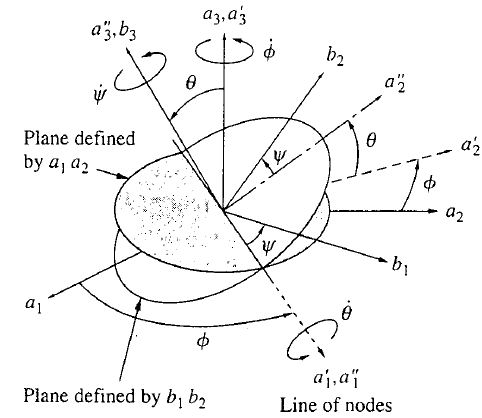
\includegraphics[scale=0.38]{apendice2fig1}
\caption{Secuencia de Euler $3-1-3$.}
\label{fig:apendice2fig1}
\end{figure}

\newpage

\section{Cuerpos con ejes de simetría} \label{app:apendice3}

\textbf{Nota}: Este apéndice es una reconstrucción de una parte de la sección 7.5.3 
de \cite{baruh}.

\vspace{.3cm}

En el estudio de los cuerpos con ejes de simetría, es más deseable describir el 
movimiento de los mismos usando un conjunto de ejes relativos que no coinciden con 
los ejes del cuerpo. Una buena opción para analizar este tipo de movimiento, 
es usar un sistema de referencia que no contenga el ángulo de espín. La motivación 
detrás de la selección de un sistema de referencia diferente al del cuerpo, 
surge del hecho de que en muchos problemas que involucran simetría axial, 
el valor del ángulo de espín no es de mucha importancia, mientras que la tasa de 
espín si lo es. Estamos más interesados en la velocidad y aceleración del centro 
de masa o de otro punto a lo largo del eje de simetría, así como en la velocidad
angular y la aceleración angular, que del movimiento de algún punto específico del 
cuerpo. En estos casos podemos decir que, la precesión y nutación describen completamente 
la orientación del eje de simetría.

\vspace{.3cm}

Consideremos una transformación $3-1-3$. Usando la notación $a_1a_2a_3$ para los 
ejes inerciales, las coordenadas asociadas con el nuevo sistema de referencia se 
convierten en los ejes $a''_1a''_2a''_3$, y podemos encontrar la velocidad angular 
luego de la rotación $3-1$ 

\begin{equation}
 {^A}{ \vec{\omega}}^{A''} = \dot{\phi}\vec{a}_3 + \dot{\theta}\vec{a}'_3 = 
 \dot{\phi}(\sen{\theta}\vec{a}''_2 + \cos{\theta}\vec{a}''_3) + \dot{\theta}\vec{a}''_1.
\label{eq:velAngFframe1}
\end{equation}

Nos referiremos a este sistema relativo, siguiendo al autor, como el marco de referencia 
$F$, con los ejes coordenados asociados $f_1f_2f_3$, y sus vectores unitarios 
$\hat{f_1}\hat{f_2}\hat{f_3}$. Para cuerpos con ejes de simetría, ver el marco de 
referencia $F$ es equivalente a ver la forma general de un disco o un trompo, sin 
seguir el movimiento de un punto específico del cuerpo. Podemos entonces escribir 
la velocidad angular del cuerpo como 

\begin{equation}
 \vec{\omega} =  {^A}{ \vec{\omega}}^{B} =  {^A}{ \vec{\omega}}^{F} + 
  {^F}{ \vec{\omega}}^{B},
  \label{eq:velAngFframe2}
\end{equation}

donde ${^A}{ \vec{\omega}}^{F} = {^A}{ \vec{\omega}}^{A''}$ y ${^F}{ \vec{\omega}}^{B}$ 
es el espín, ${^F}{ \vec{\omega}}^{B} = \dot{\psi}\hat{f}_3$. 

\vspace{.3cm}

Para una transformación $3-1-3$, podemos escribir las velocidades angulares del cuerpo 
y del marco $F$ en términos de las componentes del marco $F$ como

\begin{align}
\begin{split}
 %
 {^F}{ \vec{\omega}}^{B} &= \dot{\psi}\hat{f}_3, \\
 %
 {^A}{ \vec{\omega}}^{F} &= \dot{\phi}(\sin{\theta}\hat{a}''_2 + \cos{\theta}\hat{a}''_3) 
 + \dot{\theta}\hat{a}''_1 = \dot{\theta}\hat{f}_1 + \dot{\phi}\sen{\theta}\hat{f}_2 +
 \dot{\phi}\cos{\theta}\hat{f}_3,
 %
\end{split}
\end{align}

\begin{equation}
 \boxed{\vec{\omega} = {^A}{ \vec{\omega}}^{F} + {^F}{ \vec{\omega}}^{B} = \dot{\theta}\hat{f}_1 
 + \dot{\phi}\sen{\theta}\hat{f}_2 + (\dot{\phi}\cos{\theta} + \dot{\psi})\hat{f}_3.}
\label{eq:velAngFframe3}
\end{equation}

\newpage

\section{Tabla de la transformaciones de ángulos de Euler (específica para 3-1-3)}

\begin{figure}[H]
 \center
 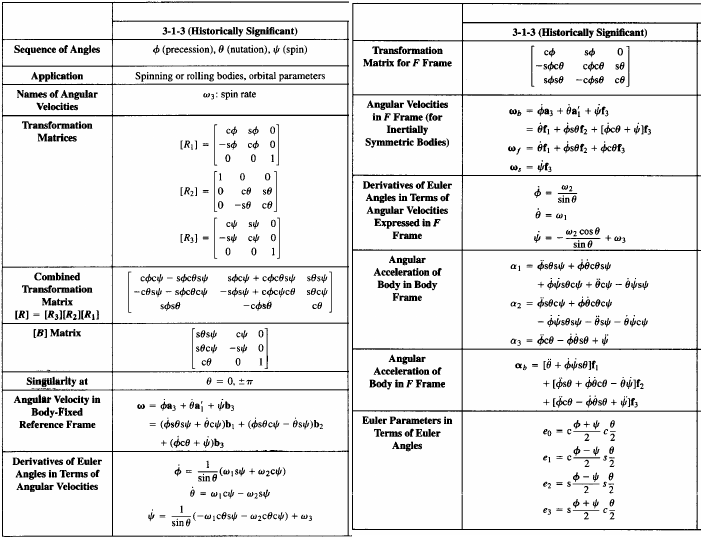
\includegraphics[scale=0.55]{apendice4fig1}
 \caption{Tomada de \cite{baruh}}
 \label{fig:apendice4fig1}
\end{figure}

\newpage

\begin{thebibliography}{20}
 \bibitem{delange}
 O. De Lange y J. Pierrus, \emph{Solved Problems on Classical Mechanics}, Oxford 
 University Press, 2010.
 \bibitem{baruh}
 H. Baruh, \emph{Analytical Dynamics}, McGraw-Hill, 1999.
 \bibitem{saletan}
 J. José y E. Saletan, \emph{Classical dynamics: A contemporary approach}, Cambridge University Press,
 1998.
 \bibitem{spivak}
 M. Spivak, \emph{Physics for mathematicians: Mechanics I}, Publish or Perish,
 2010.
 \bibitem{chaichian}
 M. Chaichian, I. Merches y A. Tureanu, \emph{Mechanics: An intensive course}, Springer-Verlang,
 2012.
 \bibitem{romano}
 A. Romano, \emph{Classical Mechanics with Mathematica\textregistered}, Birkhäuser-Springer, 
 2012.
 \bibitem{fowles}
 G. Fowles y G. Cassiday, \emph{Analytical Mechanics}, Thomson Brooks/Cole, 
 7ma edición, 2005.
 \bibitem{synge}
 J. Synge y B. Griffith, \emph{Principles of Mechanics}, 2da. edición, McGraw-Hill, 
 1949.
 \bibitem{meirovitch}
 L. Meirovitch, \emph{Methods of Analytical Dynamics}, McGraw-Hil, 1970.
 \bibitem{ginsberg1}
 J. Ginsberg, \emph{Advanced Engineering Dynamics}, Cambridge University Press 1998.
 \bibitem{ginsberg2}
 J. Ginsberg, \emph{Engineering Dynamics}, Cambridge University Press, 2008.
\end{thebibliography}


\end{document}
